
\section{Feature Evaluation}

In order produce a functioning classifier, the predictive value of the features
must be evaluated. This assesses wether a certain feature is useful in the
discrimination between formal and informal. The evaluation requires the
knowledge of what parts in a satellite image are formal and informal to create
a distinction between the two classes. This knowledge is represented in
a ground truth, this is a mask covering the satellite image indicating the
informal regions.

The mask is used to divide each block of pixels into the two classes, formal
and informal. Each block has a vector of values, also called features,
characterizing that particular block. Because the blocks are grouped together,
the features associated with the same class are grouped together as well. This
allows for the analysis of the distribution of the features in both classes. If
the distribution of a certain feature varies quite distinctly between the two
classes, this indicates as a suitable candidate for classification of informal
regions.

The groundtruth mask is constructed using a vector file containing the
boundaries of informal areas. The boundary file is rasterized and applied on
top of the satellite image, creating a mask of the informal settlements.
Because classification and feature calculation is performed on blocks instead
of pixels, the pixel based mask transformed into a block based mask. In this
mask, every pixel represents a block where the zero represents formal and one
represents informal. This effectively creates a ground truth.  

The predictive value of a feature can be visualized using a boxplot of the two
classes. When a feature is distinctive on its own, the distribution of the
values in the two classes will be different. The data used for the evaluation
comes from three small sections of the image. As priorly mentioned, this
creates a more even division of classes which should provide a more accurate
evaluation of the selected feature.

The features will be calculated for every image at different block sizes and
scales. Because block size and scale impact the predictiveness of a feature,
various combinations are used to discover the most favorable combination.

% TODO: insert concatenated image of the three sections

%Eventhough there might not be
%a significant difference between two distribution, by using multiple features
%in combination, the grand total might more distinctive that the sum of its
%parts. 

\subsection{Histogram of Oriented Gradients}

In the analysis of the historgram used block sizes of 20, 40, and 60 combined
with scales of 50, 100, 150, and 200. These combinations should capture the
difference that either an increase of block size or scale causes to the
predictiveness of a feature. For visualization purposes, only a single feature
of the 15 features of HoG of a single section is displayed here. This feature
is the most distinct between formal and informal. The other two sections are
comparable to the section used here. Moreover, not all combinations of the
block sizes and scales are presented here, only a few examples which illustrate
the distinctiveness of the features of the Histogram of Oriented Gradients.

\begin{figure}
\begin{tabular}{cc}
  \subfloat{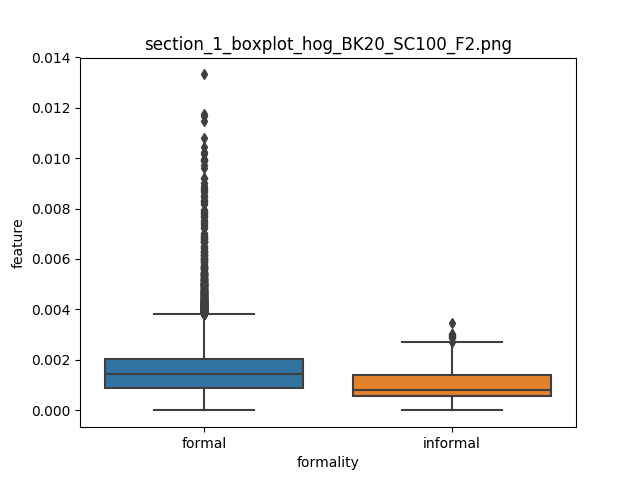
\includegraphics[width=4cm]{images/HoG/inc_bk/section_1_boxplot_hog_BK20_SC100_F2}}&
  \subfloat{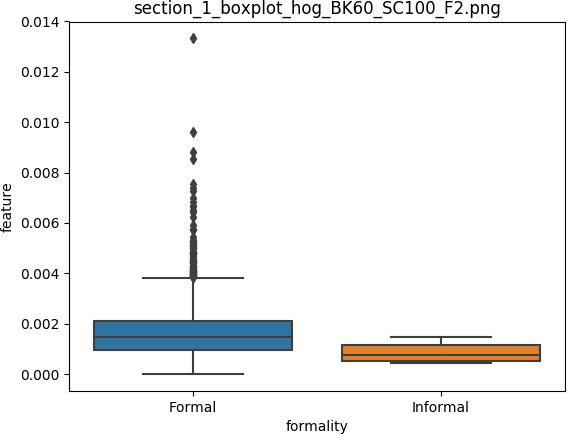
\includegraphics[width=4cm]{images/HoG/inc_bk/section_1_boxplot_hog_BK60_SC100_F2}}\\ 
  \subfloat{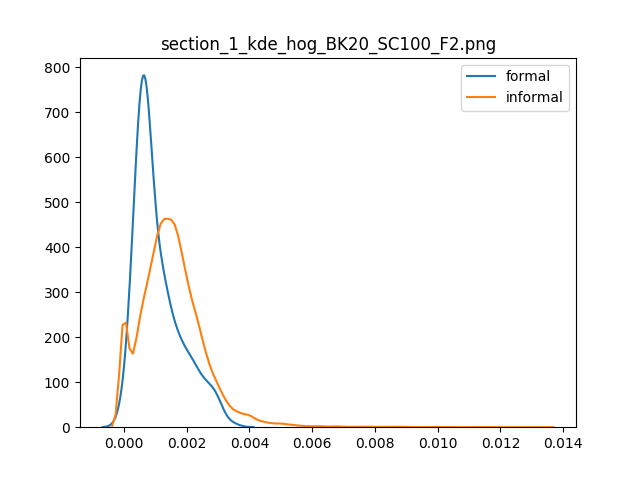
\includegraphics[width=4cm]{images/HoG/inc_bk/section_1_kde_hog_BK20_SC100_F2}}&
  \subfloat{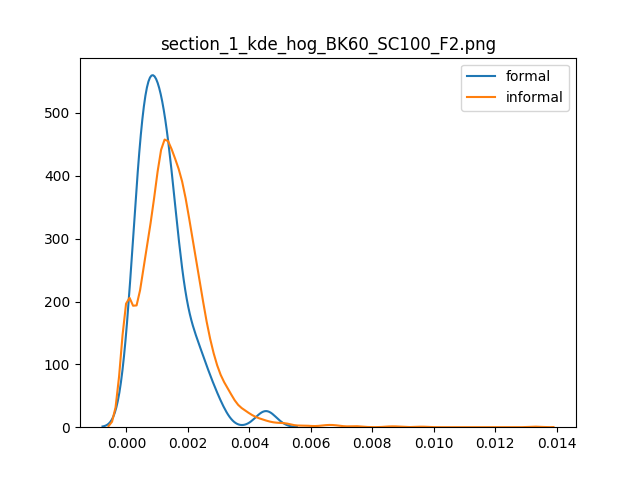
\includegraphics[width=4cm]{images/HoG/inc_bk/section_1_kde_hog_BK60_SC100_F2}}
\end{tabular}
\caption{The effect of increased block size on a HoG feature. From left to
right: a block size of 20 and 60 respectively.}
\label{hog_inc_bk}
\end{figure}

Figure \ref{hog_inc_bk} shows the effect that an increased block size has on
the distribution of values in both classes. This example uses a constant scale
of 100 pixels and a variable block size of 20 and 60 pixels. The experiment
with a block size of 40 is performed as well, but is ommited from the figure to
keep the results brief. A more comprehensive visualization of the evaluation
can be found in the appendix. It seems that the block size, in this case, does
not influence the both distrutions significantly. As a result an increase in
the size of a block will have little influence on the predictive value of the
HoG.

\begin{figure}
\begin{tabular}{cc}
  \subfloat{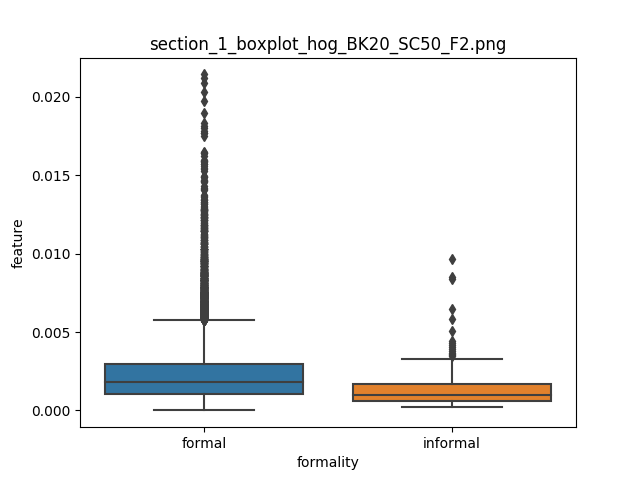
\includegraphics[width=4cm]{images/HoG/inc_sc/section_1_boxplot_hog_BK20_SC50_F2}}&
  \subfloat{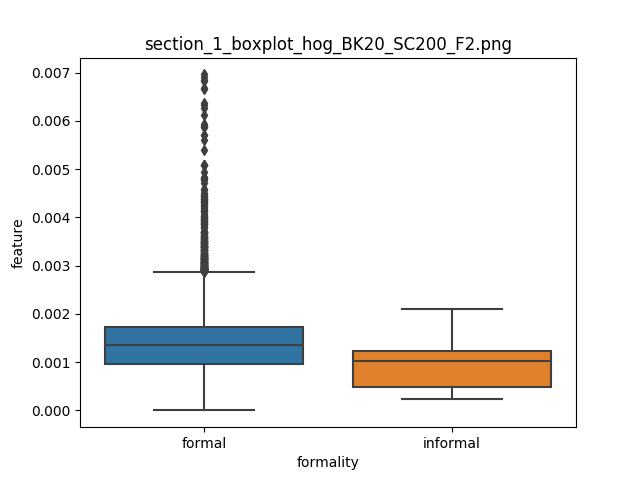
\includegraphics[width=4cm]{images/HoG/inc_sc/section_1_boxplot_hog_BK20_SC200_F2}}\\
  \subfloat{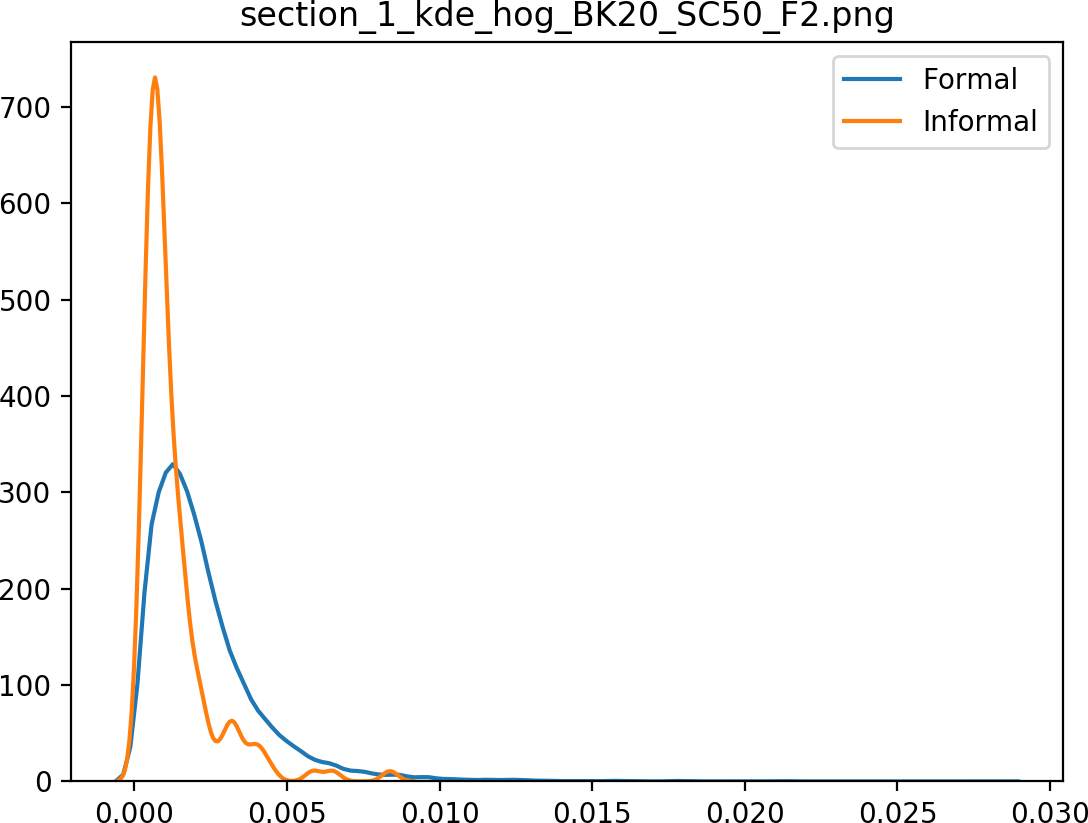
\includegraphics[width=4cm]{images/HoG/inc_sc/section_1_kde_hog_BK20_SC50_F2}}&
  \subfloat{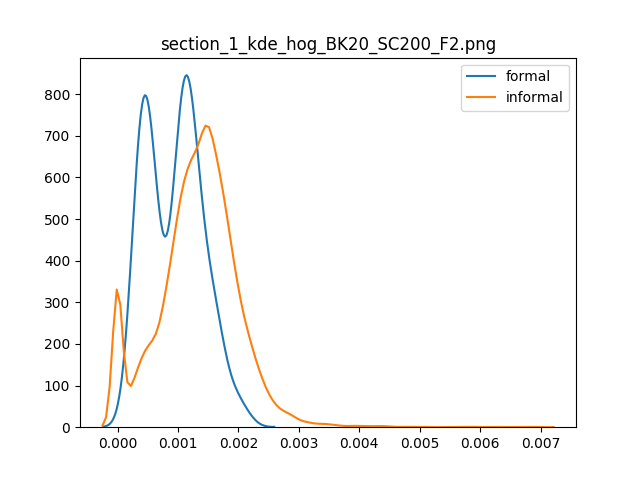
\includegraphics[width=4cm]{images/HoG/inc_sc/section_1_kde_hog_BK20_SC200_F2}}\\
\end{tabular}
\caption{The effect of increased scale on a HoG feature. From left to
right: a scale of 50 and 200 respectively}
\label{hog_inc_sc}
\end{figure}

Figure \ref{hog_inc_sc} illustrates the effect of increased scale on a constant
block size. It seems to indicate that an increased scale leads to an increased
separatation of the two distribution, thus increasing the predictiveness of the
feature.

\subsection{Line Support Region}

Similar to the analysis of the Histogram of Oriented Gradients, the analysis of
Line Support Region uses a combination of different block sizes and scales.
Unlike HoG, however, the scale 200 is not included due to the high
computational cost. 
